\documentclass[11pt,a4paper]{article}
\usepackage{fontspec}
\setmainfont{TeX Gyre Pagella}
\newfontfamily\headfont{Inter}[UprightFont=*-ExtraBold,BoldFont=*-ExtraBold,Extension=.otf,Path=/usr/share/fonts/opentype/inter/]
\usepackage[a4paper,margin=2.3cm]{geometry}
\usepackage{graphicx,booktabs,float,caption,array,xcolor,longtable}
\usepackage{xurl}
\usepackage[hidelinks]{hyperref}
\usepackage{titlesec}
\usepackage[round]{natbib}
\usepackage{setspace}
\setstretch{1.05}
\renewcommand{\topfraction}{0.9}
\renewcommand{\bottomfraction}{0.8}
\renewcommand{\textfraction}{0.1}
\renewcommand{\floatpagefraction}{0.75}
\setlength{\parindent}{0pt}
\setlength{\parskip}{0.55em}
\titleformat{\section}{\headfont\Large}{\thesection}{0.8em}{}
\titleformat{\subsection}{\headfont\large}{\thesubsection}{0.8em}{}
\captionsetup{font=small,labelfont=bf}
\urlstyle{same}
\hypersetup{pdftitle={Transported},pdfauthor={Tristan Hotham}}

\begin{document}
\begin{center}
{\Large\bfseries Transported\par}
\vspace{0.4em}
{\large The convict ships to Australia, 1788 to 1868, and the wider world of penal transportation:\\745 voyages in Wikipedia's ship lists\par}
\vspace{1.2em}
{\large Tristan Hotham\par}
\vspace{0.3em}
{\small Independent researcher\\
ORCID: 0000-0003-4931-9349\\
DOI: https://doi.org/10.5281/zenodo.23873537\par}
\vspace{0.8em}
2026
\end{center}

\begin{quote}
\small
\begin{center}\textbf{Abstract}\end{center}
Britain transported about 162,000 convicts to Australia between 1788 and 1868. I assemble English Wikipedia's four colony lists of convict ships into a single table of 834 listed voyages and map the 745 that arrived from overseas, 92\% of the 806 ships the articles give. Arrivals rose from a handful a year to a peak of 35 in 1833; 76\% came between 1815 and 1840. Cork was the busiest single port of departure (101 voyages), and Irish ports supplied 26\% of the voyages from the British Isles, but 34\% of those to New South Wales against 6\% of those to Van Diemen's Land. A further 101 voyages sailed from India, Ceylon, Mauritius and Singapore. For the 53 voyages with both dates in the fleet tables or ship articles, the median passage fell from 190 days for the first three fleets to 115 in the 1820s and 1830s. The Second Fleet lost 26\% of its embarked convicts at sea and the Third Fleet 8.8\%, against 0.8\% on 24 later voyages whose ship articles give both figures. The lists give convict numbers for only 108 voyages (21,871 people), almost none for New South Wales and Tasmania, and identify only 20 women's voyages, so they map the shipping well but cannot count the people. Set beside the articles' figures for British America, French Guiana, New Caledonia, Russia's katorga and the Andaman Islands, the Australian system was the largest and longest of its kind.

\textbf{Keywords:} penal transportation; convicts; Australia; convict ships; maritime history; colonial history; Wikipedia; open data; mapping
\end{quote}

\section{Introduction}
Penal transportation, the shipping of convicted people to distant colonies to serve their sentences, was used by several European empires from the seventeenth to the twentieth century \citep{wiki}. Britain's use of it was the largest: first to the American colonies under the Transportation Act of 1717, and then, after the American Revolution closed that route in 1776, to the Australian colonies, where about 162,000 convicts from Great Britain and Ireland arrived between 1788 and 1868. The colonies were founded on Aboriginal land: the First Fleet met the Eora people at Sydney Cove, and Wikipedia's article on penal transportation records that violent conflict on the Australian frontier ``began only months after the First Fleet landed, lasting over a century''.

The voyages themselves are well documented, above all in Charles Bateson's \emph{The Convict Ships}, and English Wikipedia's volunteers have compiled lists of them, colony by colony. This paper asks what those lists, taken together, can and cannot tell us: how many voyages they hold and when, where the ships sailed from, how long they took and how many convicts died, and how the Australian system compares with other penal transportation systems described in the same encyclopaedia. The paper accompanies an interactive map (\url{https://maps.tristanhotham.com/transported-convicts/}).

\section{Data}
\textbf{Voyage lists.} ``Convict ships to New South Wales'' (604 rows, including one added below) and ``Convict ships to Tasmania'' (147) give, for each voyage, the ship's name with a link to its article where one exists, the date of arrival, the place it sailed from and brief notes. Neither gives the number of convicts or a departure date. ``Convict ships to Norfolk Island'' (33 arrivals) gives convicts embarked and landed, both for the transfers from Sydney in 1788 to 1804 and for ships that sailed direct from Britain and Ireland in 1840 to 1850. ``List of convict ship voyages to Western Australia'' (50 rows) gives the origin, arrival and number of convicts for the 43 voyages of 1850 to 1868, and the number of boys for 7 ships of 1842 to 1849 that carried Parkhurst apprentices.

\textbf{Fleets and ships.} The articles on the First, Second and Third Fleets have per-ship tables with departure and arrival dates, voyage length and convicts, and for the Third Fleet deaths. For 305 ship articles in Wikipedia's convict ship categories I read the infobox (launch year, tons burthen) and lead, and for the ships whose full article was available I read sentences giving a departure date, an arrival date, convicts embarked and convict deaths.

\textbf{Context.} Totals and dates for the Australian system and for other penal transportation systems come from the articles listed in Table~\ref{tab:revs}. Every figure quoted is checked in the code against the exact phrase in the article. No article text is reproduced beyond short quotations. Land outlines are from Natural Earth \citep{naturalearth}.

\section{Method}
\textbf{Voyages.} A listed voyage is one row of the four lists. The New South Wales list omits Prince of Wales, a First Fleet transport, which I add from the First Fleet article. A \emph{voyage from overseas} is a row with an arrival year whose departure place lies outside Australia, excluding the 7 Parkhurst apprentice ships (234 boys, matching the article's 234) and 15 voyages listed by two colonies, identified as the same ship name arriving in both within 75 days (for example a ship that landed convicts at Hobart and then sailed on to Sydney). Such a voyage is kept once, in the list that gives a number of convicts or else at its first arrival. The 57 transfers between Australian ports and the 10 rows without an arrival year (wrecks, a capture, ships listed without dates) are kept in the data but not counted. Years are years of arrival.

\textbf{Departure places.} The ``sailed from'' cell is matched to one of 38 places, with coordinates I chose for each harbour or anchorage. Where a cell names two places the first is taken as the port of departure. ``England'' and ``Ireland'' without a port are kept as such (62 voyages give only ``England''). Ireland comprises Cork, Dublin (Kingstown), Waterford and ``Ireland''.

\textbf{Numbers, dates and deaths.} The number of convicts on a voyage is the number landed where given and otherwise the number embarked. Fleet ships are matched to the New South Wales list by name and year. A ship article's voyage is kept only if its arrival date is within 3 days of a list row for the same ship; the first departure date in the article's account is used (later sentences often describe calls at Tenerife or Rio de Janeiro). Voyage length is the fleet table's stated duration or the difference between the article's two dates.

\textbf{Women's voyages.} A voyage is flagged as carrying women where a fleet table or ship article gives female convicts, where the list's notes mention them, or where a ship article sentence says the ship carried female convicts in a year matching exactly one of its voyages (and not male convicts too).

\textbf{Routes.} The lists record no tracks. Each voyage is drawn on a stylised route through open-sea waypoints chosen to follow the usual pattern of the period: south past Madeira and the Cape Verde islands, west towards Brazil, east across the South Atlantic and south of the Cape of Good Hope, then along the Southern Ocean to Fremantle, round the south of Van Diemen's Land to Hobart, or up the east coast to Sydney and Norfolk Island. Ships from India, Mauritius and Singapore cross the Indian Ocean and pass through Bass Strait. Every route is checked not to cross Natural Earth land.

\begin{table}[tbp]\centering\footnotesize\setlength{\tabcolsep}{4pt}\caption{Listed voyages from overseas by colony: first and last arrival, busiest year, voyages with a number of convicts and the convicts they carried, voyages from Ireland and from India and the Indian Ocean, and (not counted) transfers within Australia.}\label{tab:colonies}\begin{tabular}{lrrrrrrrrr}\toprule Colony & Voyages & First & Last & Busiest & With no. & Convicts & Ireland & India etc. & Transfers\\\midrule
New South Wales & 556 & 1788 & 1849 & 1829 (27) & 44 & 7,993 & 152 & 95 & 34\\
Van Diemen's Land & 132 & 1812 & 1852 & 1830 (9) & 7 & 1,459 & 7 & 0 & 4\\
Norfolk Island & 14 & 1840 & 1850 & 1840 (3) & 14 & 2,745 & 3 & 0 & 19\\
Western Australia & 43 & 1850 & 1868 & 1858 (5) & 43 & 9,674 & 1 & 6 & 0\\
\midrule All & 745 & 1788 & 1868 & 1833 (35) & 108 & 21,871 & 163 & 101 & 57\\
\bottomrule\end{tabular}\end{table}

\section{Results}
\subsection{Eighty years of voyages}
Figure~\ref{fig:map} maps the 745 voyages and Figure~\ref{fig:years} counts them by year. The First Fleet's 6 transports arrived in 1788; the 1790s, with the Second and Third Fleets, had 30 voyages, and the war years were thin: 32 in the 1800s. Arrivals rose steeply after 1815. The 1820s had 206 and the 1830s 264, with a peak of 35 in 1833; 567 voyages (76\%) arrived between 1815 and 1840. New South Wales received 556 voyages and peaked at 27 in 1829. Transportation there was suspended in 1840 and formally abolished on 1 October 1850; the list's last arrival is Adelaide, 24 December 1849. From 1841 to 1849 the lists hold 16 arrivals in Van Diemen's Land, 10 at Norfolk Island and 5 in New South Wales. The Tasmania list ends with Sir Robert Seppings on 8 July 1852, while its introduction names St Vincent, 26 May 1853, as the last. Western Australia's 43 voyages ran from Scindian in 1850 to Hougoumont in 1868.

\begin{figure}[tbp]\centering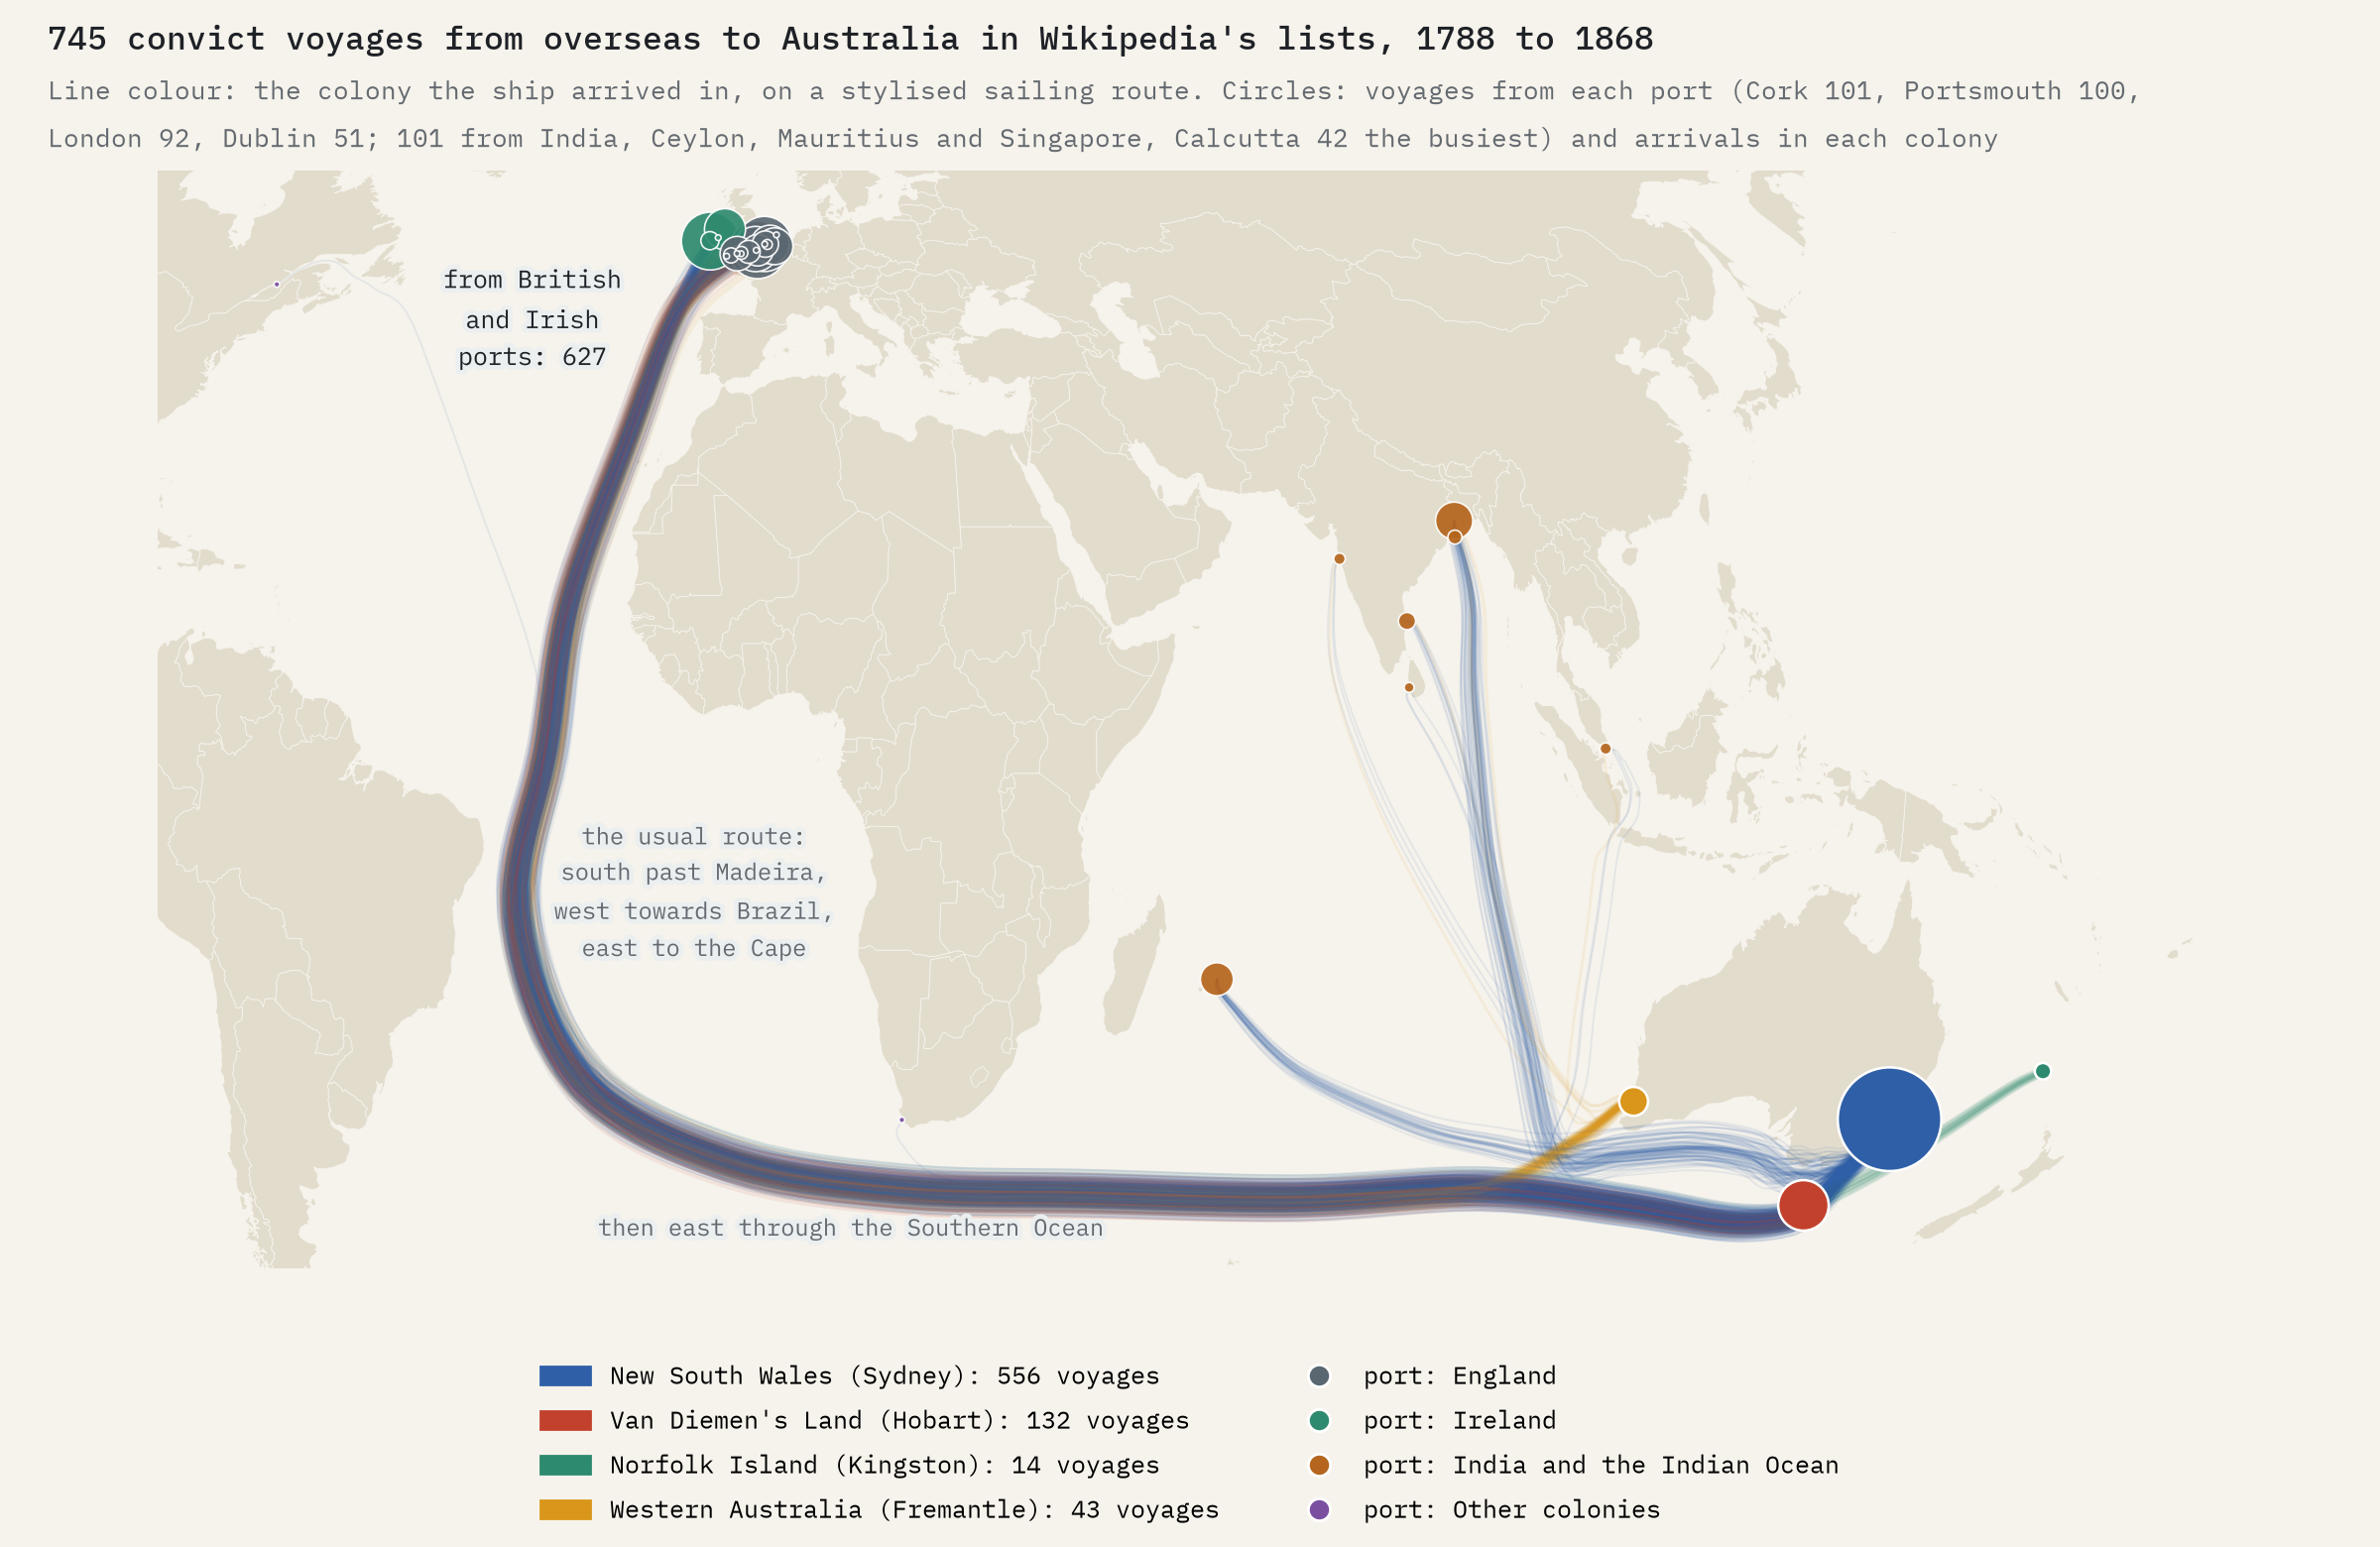
\includegraphics[width=\textwidth]{f_map.png}
\caption{Convict voyages from overseas in Wikipedia's lists, on stylised sailing routes, coloured by colony. Circles: voyages from each port.}\label{fig:map}\end{figure}

\begin{figure}[tbp]\centering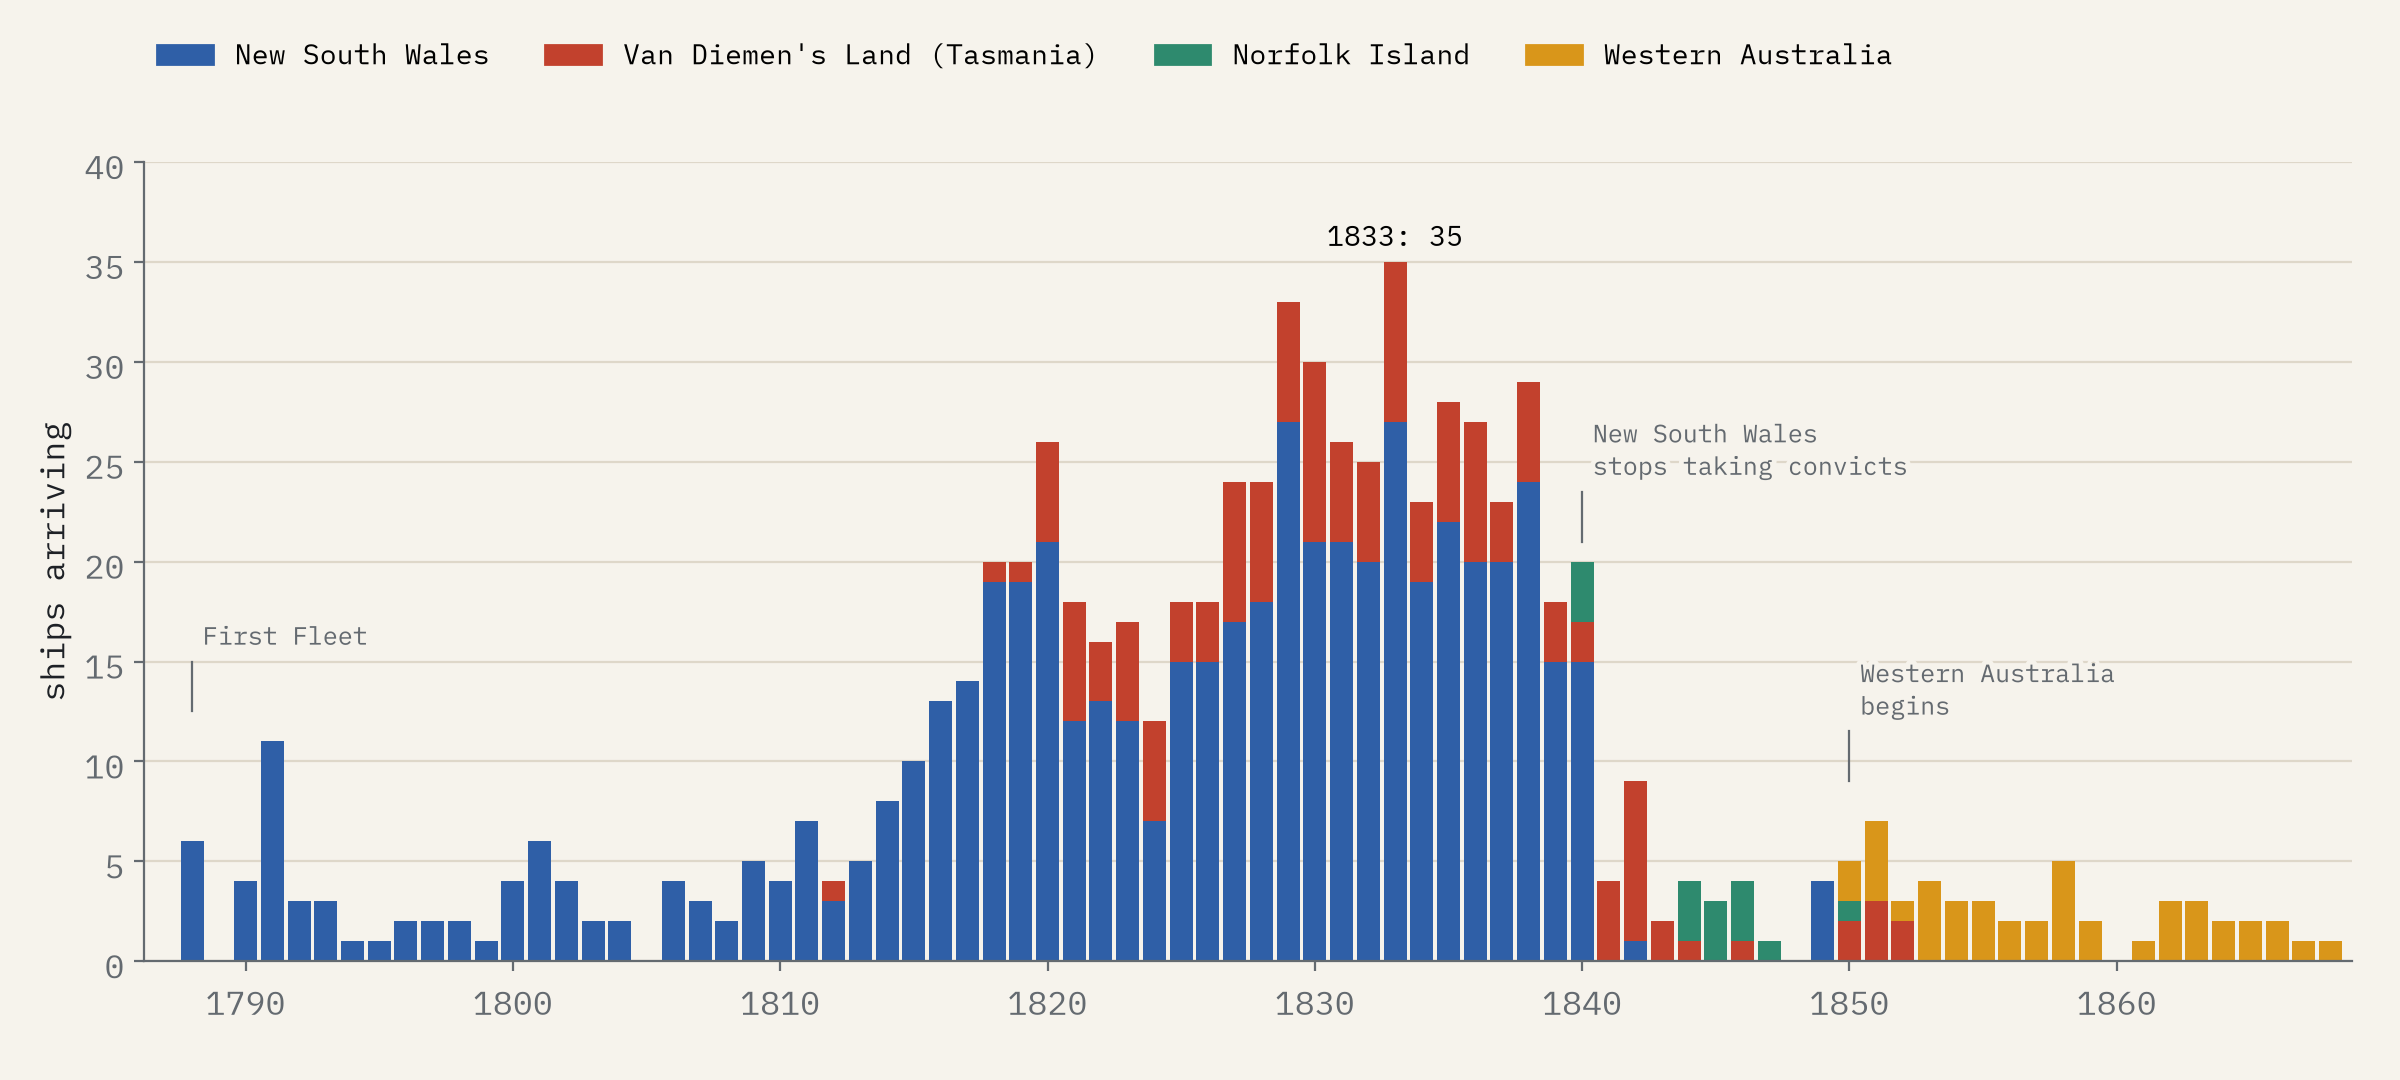
\includegraphics[width=\textwidth]{f_years.png}
\caption{Convict ships arriving from overseas, by year and colony.}\label{fig:years}\end{figure}

\subsection{How complete are the lists?}
The articles give about 162,000 convicts (``Convicts in Australia'' also gives ``about 164,000 \ldots onboard 806 ships''). The lists' 745 voyages are 92\% of 806. Numbers of convicts are given for 108 voyages (14.5\%), 21,871 people or 13.5\% of 162,000: all 43 Western Australian voyages, the 14 direct voyages to Norfolk Island, and 44 New South Wales and 7 Tasmanian voyages from the fleet tables and ship articles (Figure~\ref{fig:cover}). Those voyages carried a mean of 203 convicts, equal to the 203 implied by 164,000 over 806; at that mean the listed voyages would account for about 151,000 people. Western Australia's list is complete: its 43 voyages sum to 9,674, between the 9,668 and 9,721 given by two articles.

\begin{figure}[tbp]\centering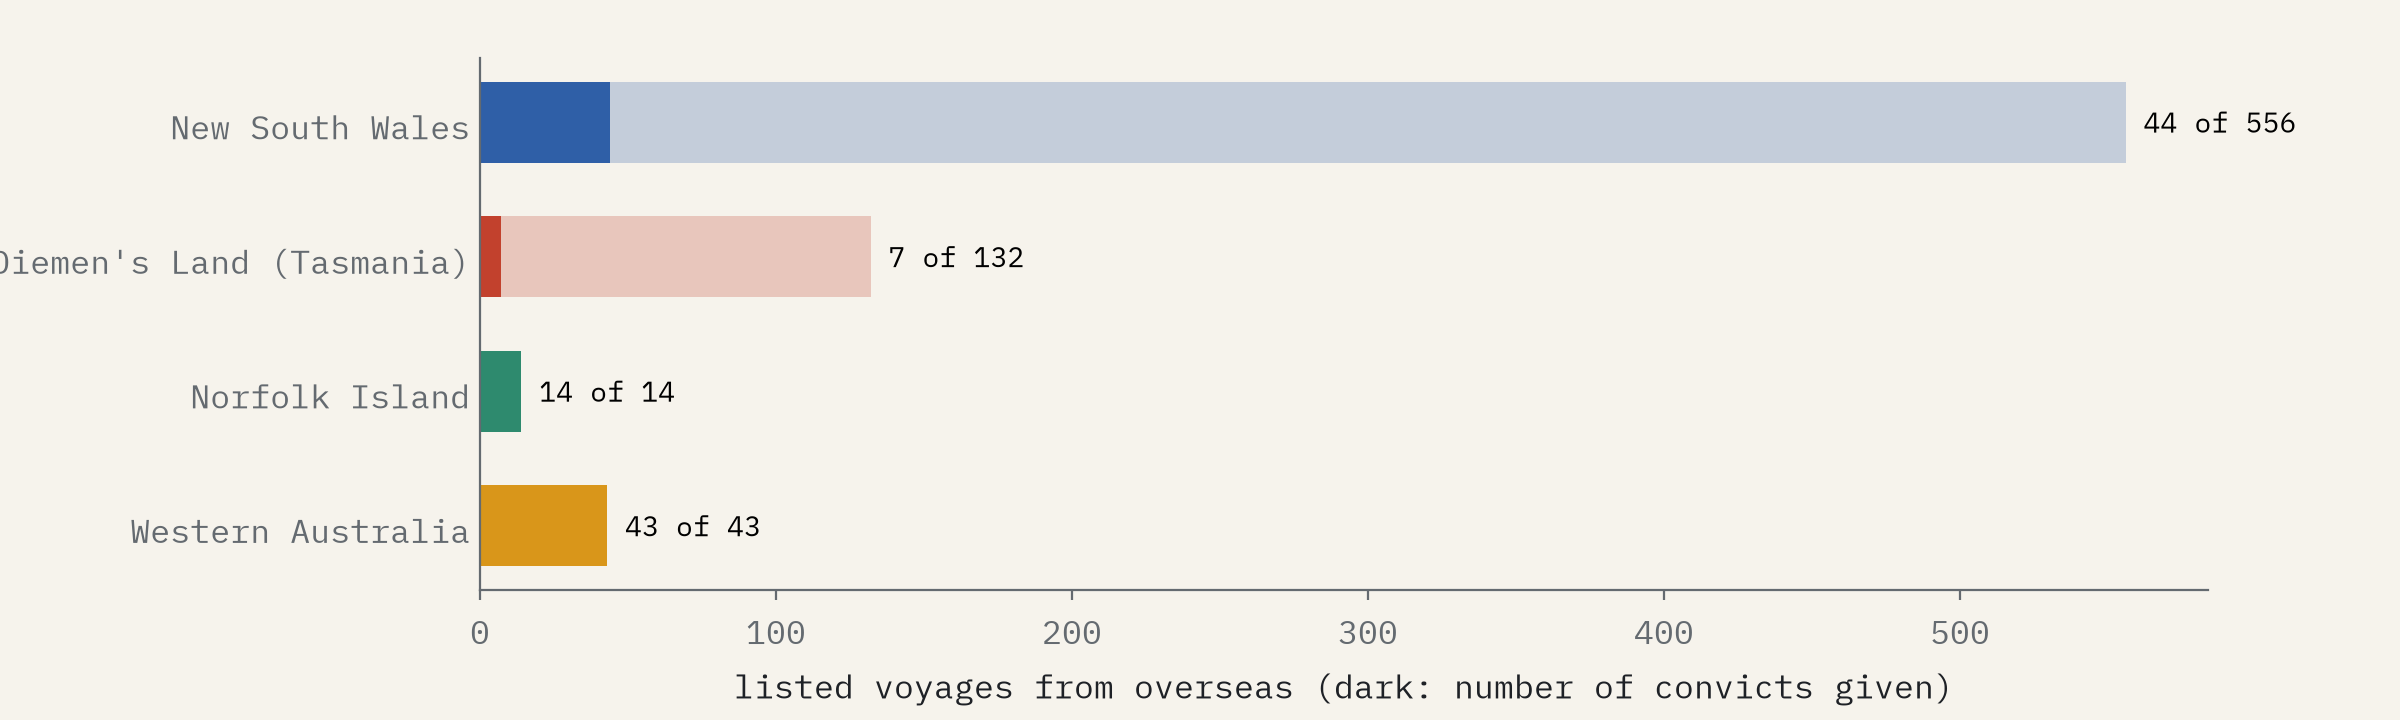
\includegraphics[width=\textwidth]{f_cover.png}
\caption{Listed voyages from overseas by colony; dark: voyages with a number of convicts in a table or ship article.}\label{fig:cover}\end{figure}

\subsection{Where the ships sailed from}
Of the 627 voyages from Britain and Ireland, 203 left from the Thames and the Downs (London, Woolwich, Deptford, Gravesend, Sheerness) and 131 from Portsmouth and Spithead, but the busiest single place in the lists is Cork, with 101 (Figure~\ref{fig:ports}). Irish ports supplied 163 voyages (26.0\%). Almost all went to New South Wales (152, or 33.8\% of that colony's voyages from the British Isles), against 7 to Van Diemen's Land (5.5\%) and 1 to Western Australia, whose ships sailed most often from Portland (15) and Plymouth (9). The 101 voyages from India, Ceylon, Mauritius and Singapore (13.6\%, 1807 to 1859) went almost all to New South Wales (95); the 6 to Western Australia carried 38 convicts between them, and 15 New South Wales notes mention military convicts.

\begin{figure}[tbp]\centering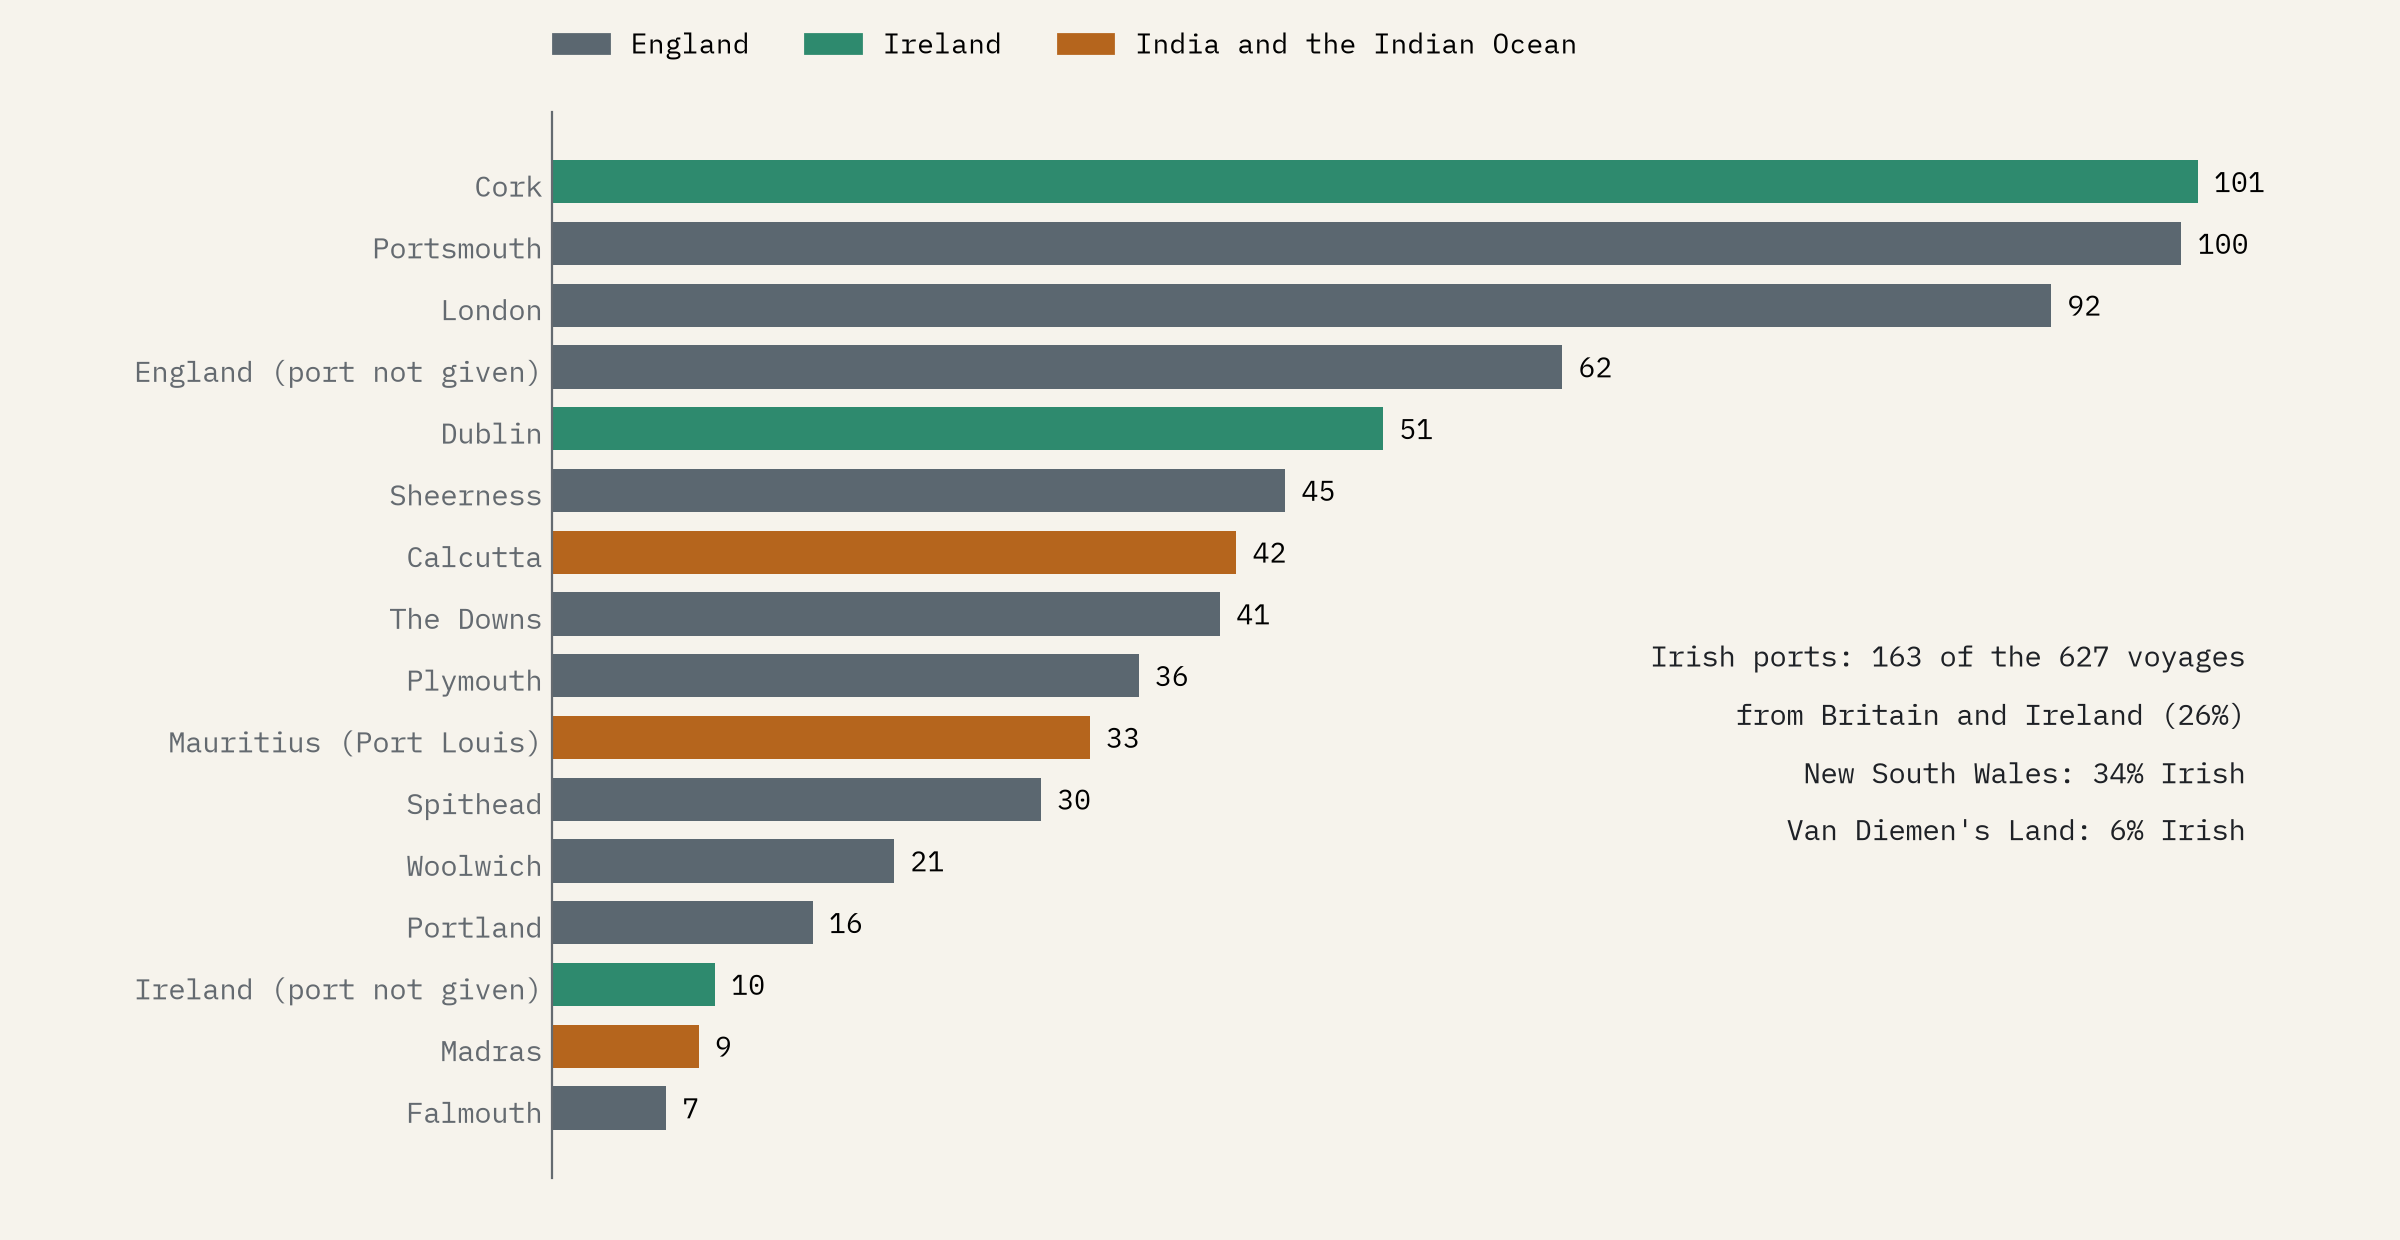
\includegraphics[width=\textwidth]{f_ports.png}
\caption{The busiest ports of departure.}\label{fig:ports}\end{figure}

\subsection{The passage}
For 53 voyages the departure and arrival are both known: 21 from the fleet tables and 32 from ship articles (Figure~\ref{fig:days}). The medians by period are 190 days for 1787 to 1791 (21 voyages), 164 for 1800 to 1819 (5), 115 for 1820 to 1839 (24) and 90 for 1840 to 1868 (3). The longest passage is Lady Juliana's 309 days in 1790; after the fleets, Friends took 262 days in 1811, sailing via Rio de Janeiro. The shortest is Scindian's 89 days in 1850; Hougoumont's last voyage took 90 by the article's dates. The sample after 1840 is very small and the sample before 1820 nearly as small, so the decline is clearer between the fleets and the 1820s than after.

\begin{figure}[tbp]\centering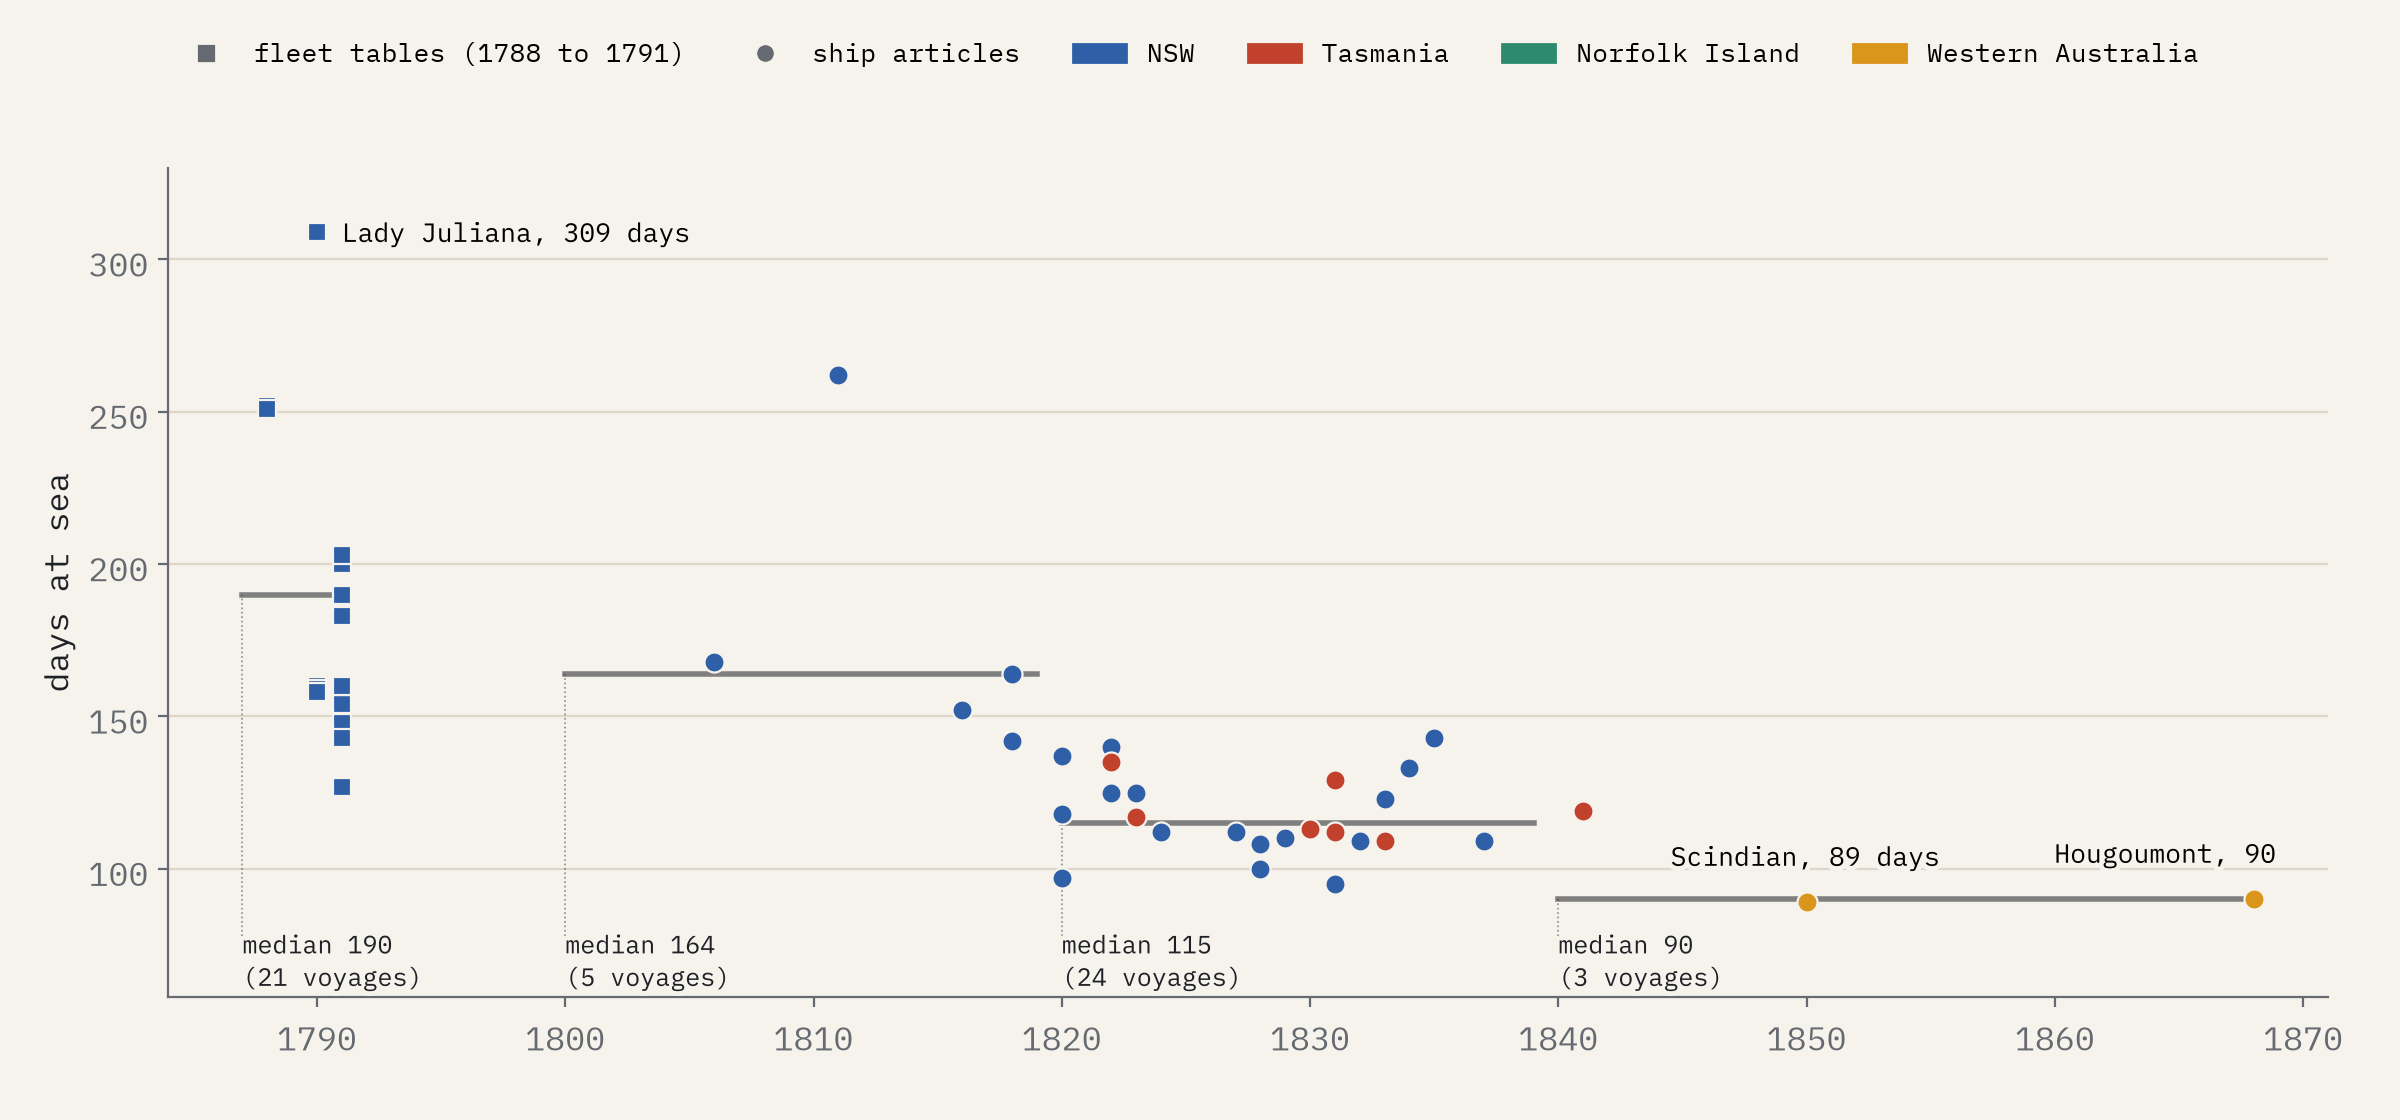
\includegraphics[width=\textwidth]{f_days.png}
\caption{Days from departure to arrival, where both dates are known. Lines: medians by period.}\label{fig:days}\end{figure}

\subsection{Deaths at sea}
The Second Fleet article gives 273 deaths among 1,038 convicts embarked (26\%), 486 landed sick and 124 more dead soon after; the article on convict women gives 267 deaths among 1,006. Its contractors were paid per head ``whether they landed alive or not''. The Third Fleet table gives 182 deaths among 2,067 boarded (8.8\%), from 3.1\% on Salamander to 14.0\% on Britannia (Figure~\ref{fig:deaths}). The First Fleet's surgeon reported 48 deaths and 28 births on the voyage. For 24 later voyages the ship articles give both the number embarked and the convict deaths: 37 of 4,765 (0.8\%), with no deaths on 9 and at most 6 (Tellicherry, 1806). These later voyages are a convenience sample of well documented ships, not a random one. The lists also record wrecks: Amphitrite, lost at the outset of her voyage with 108 women convicts and 12 children, Neva with 224 lives, and George III before she could land her convicts.

\begin{figure}[tbp]\centering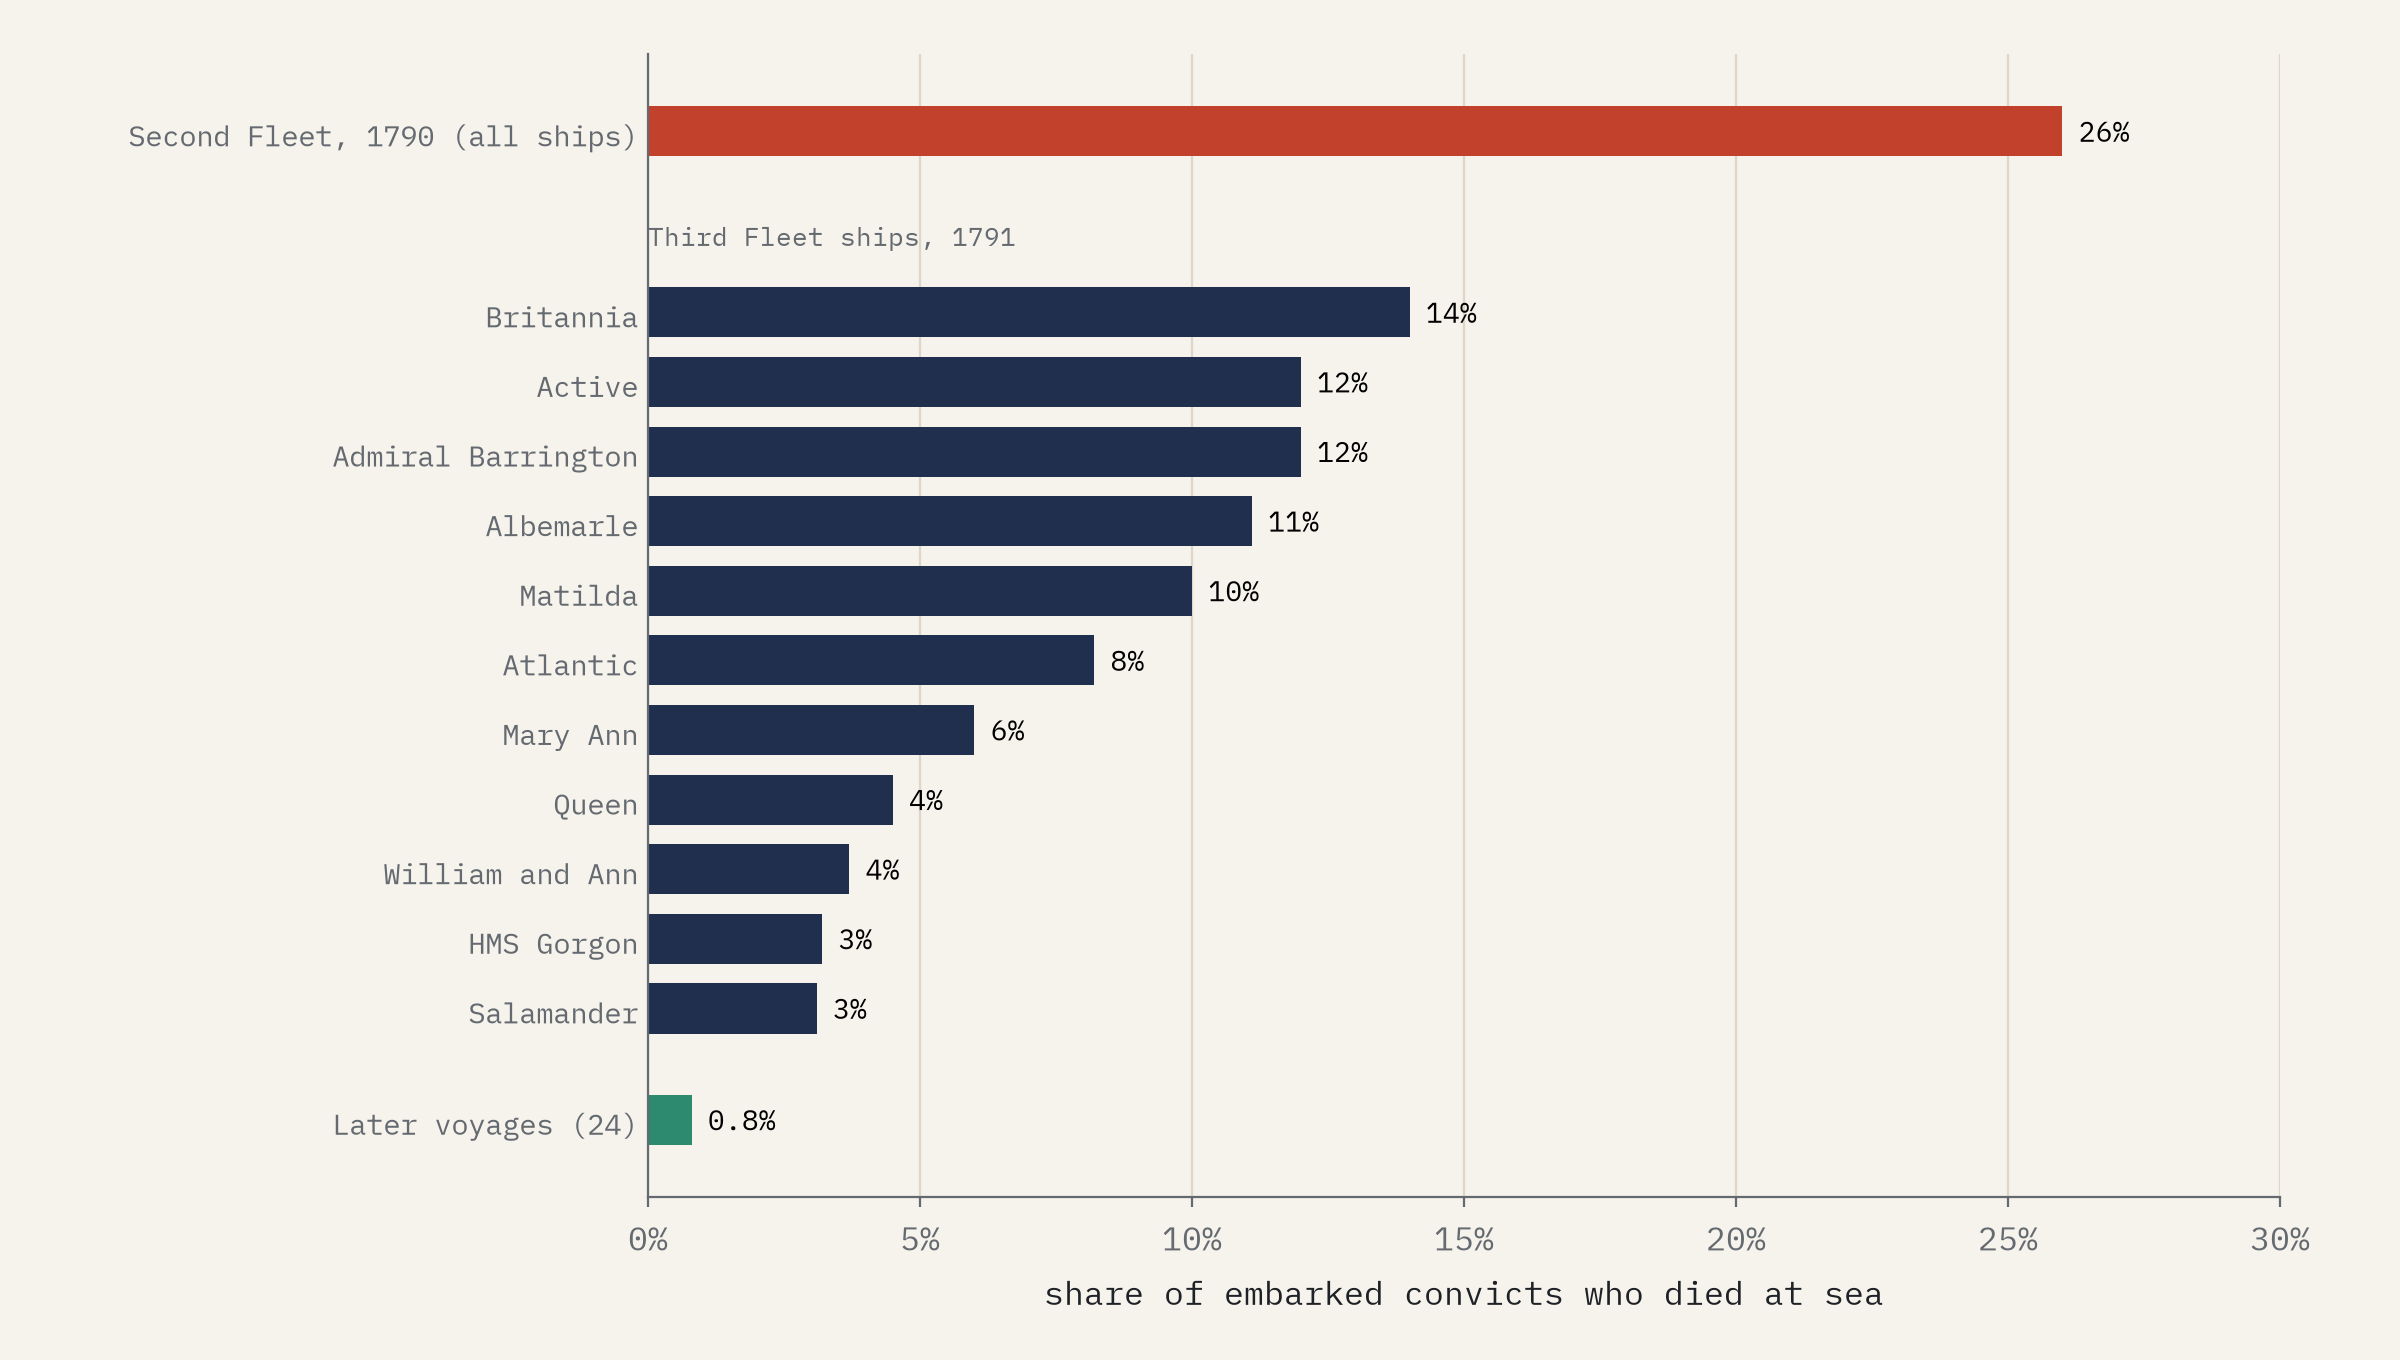
\includegraphics[width=\textwidth]{f_deaths.png}
\caption{Share of embarked convicts who died at sea.}\label{fig:deaths}\end{figure}

\subsection{Ships}
The voyages from overseas were made by 453 ships (grouped by article, or by name within a list where there is no article), 296 of them making a single listed voyage. Table~\ref{tab:ships} lists those with the most. For 121 of the 144 ships whose article states a number of convict voyages, the lists hold that number. Where the article gives a launch year, the median ship was 14 years old at arrival (503 voyages); the median tons burthen of the 260 ships with one is 443.

\begin{table}[tbp]\centering\small\caption{Ships with the most listed convict voyages from overseas, with the launch year and the number of convict voyages stated in the ship's own article where given.}\label{tab:ships}\begin{tabular}{lrllrr}\toprule Ship & Voyages & Years & Colonies & Launched & Article says\\\midrule
Mangles & 9 & 1820 to 1840 & NSW, Norfolk Island, Tasmania & 1803 & 9\\
Guildford & 8 & 1812 to 1829 & NSW & 1810 & \\
Surrey & 8 & 1816 to 1840 & NSW &  & \\
Asia & 8 & 1820 to 1836 & NSW, Tasmania & 1818 & 8\\
Eliza & 6 & 1820 to 1832 & NSW, Tasmania & 1802 & 5\\
Norfolk & 6 & 1825 to 1837 & NSW, Tasmania & 1814 & 4\\
John & 6 & 1827 to 1837 & NSW, Tasmania & 1809 & \\
Waterloo & 6 & 1829 to 1838 & NSW, Tasmania & 1815 & 4\\
Canada & 5 & 1801 to 1819 & NSW & 1800 & 5\\
Morley & 5 & 1817 to 1829 & NSW, Tasmania & 1811 & 6\\
Isabella & 5 & 1818 to 1833 & NSW, Tasmania & 1818 & 6\\
Minerva & 5 & 1818 to 1839 & NSW & 1805 & 4\\
\bottomrule\end{tabular}\end{table}

\subsection{Women}
About 24,000 of the convicts, one in seven, were women; some 80\% had been convicted of theft, and none for prostitution, which was not a transportable offence. Only 20 voyages can be identified from the lists as carrying women, a floor rather than an estimate: during the 25 years of Elizabeth Fry's involvement alone, 12,000 women came on 106 ships. The article's table of the convict population of New South Wales (Figure~\ref{fig:women}) shows women's share falling from 26.2\% in 1788 to 11.6\% in 1841. Western Australia set the condition that no women be sent.

\begin{figure}[tbp]\centering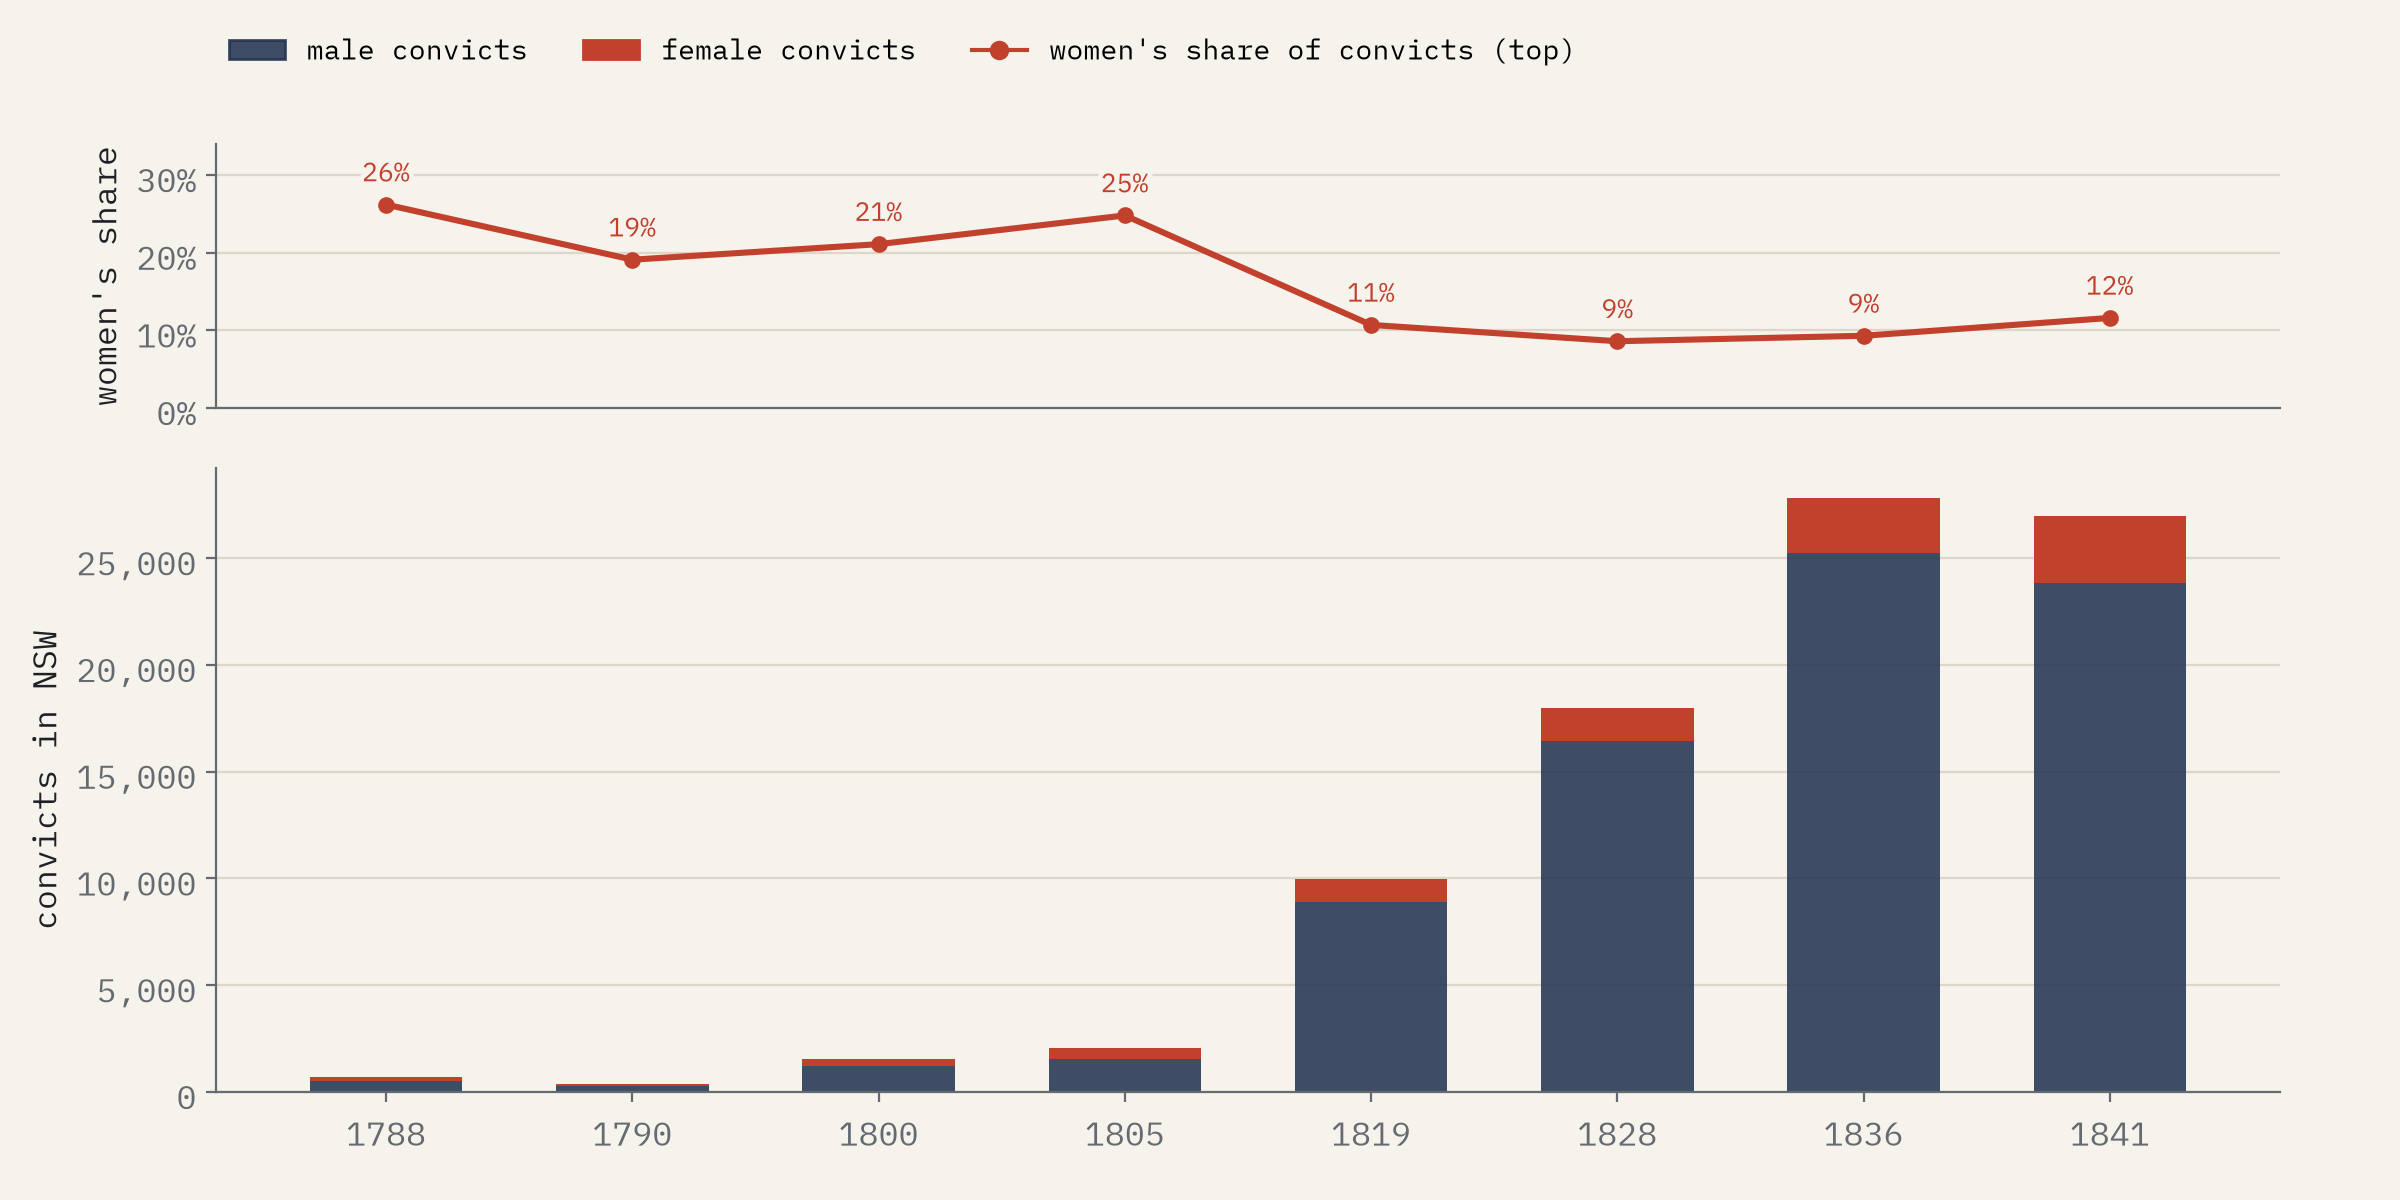
\includegraphics[width=\textwidth]{f_women.png}
\caption{Convict population of New South Wales by sex.}\label{fig:women}\end{figure}

\subsection{The wider world}
Table~\ref{tab:world} and Figure~\ref{fig:world} set the Australian voyages beside other systems, using only figures the articles state. Transportation to British America, 1718 to 1776, is ``commonly accepted'' to have taken 30,000, with estimates of 50,000 to 120,000. France sent more than 80,000 prisoners to the Devil's Island system in French Guiana (1852 to 1953) and about 22,000 to New Caledonia (1864 to 1897). Russia's katorga had about 6,000 serving in 1906 and up to 28,600 by 1916, and a penal colony on Sakhalin from 1857. British India's penal settlement in the Andaman Islands received its first 200 convicts in 1858 and closed in 1947; one article puts the number of political prisoners sent to the Cellular Jail at an estimated 80,000, a figure I report but cannot check. Bermuda's convict hulks (1823 to 1863) and Sakhalin have no total in these sources.

\begin{table}[tbp]\centering\footnotesize\setlength{\tabcolsep}{4pt}\caption{Penal transportation systems in the articles, with the numbers they state. For Sakhalin and Siberia the articles used give a start but no end.}\label{tab:world}\begin{tabular}{p{2.4cm}p{1.9cm}p{2.3cm}p{4.0cm}p{4.0cm}}\toprule Destination & From & Years & Convicts, as stated & Articles\\\midrule
Australia & Britain and Ireland & 1788 to 1868 & about 162,000 & Convicts in Australia\\
British America & Britain & 1718 to 1776 & 30,000 to 50,000; estimates range to 120,000 & Convicts in Australia; Transportation Act 1717\\
Bermuda & Britain & 1823 to 1863 & not stated & Penal transportation; Royal Naval Dockyard, Bermuda\\
French Guiana & France & 1852 to 1953 & more than 80,000 & Bagne (penal establishment); Devil's Island; Penal transportation\\
New Caledonia & France & 1864 to 1897 & about 22,000 & Bagne (penal establishment); Penal transportation\\
Andaman Islands & British India & 1858 to 1947 & 200 in the first party, 1858; the Cellular Jail had 698 cells & Andaman Islands; Penal transportation; Port Blair\\
Sakhalin & Russia & from 1857 & not stated & Katorga; Sakhalin\\
Siberia & Russia & from the 17th century & about 6,000 serving katorga in 1906, up to 28,600 by 1916 & Gulag; Katorga\\
\bottomrule\end{tabular}\end{table}

\begin{figure}[tbp]\centering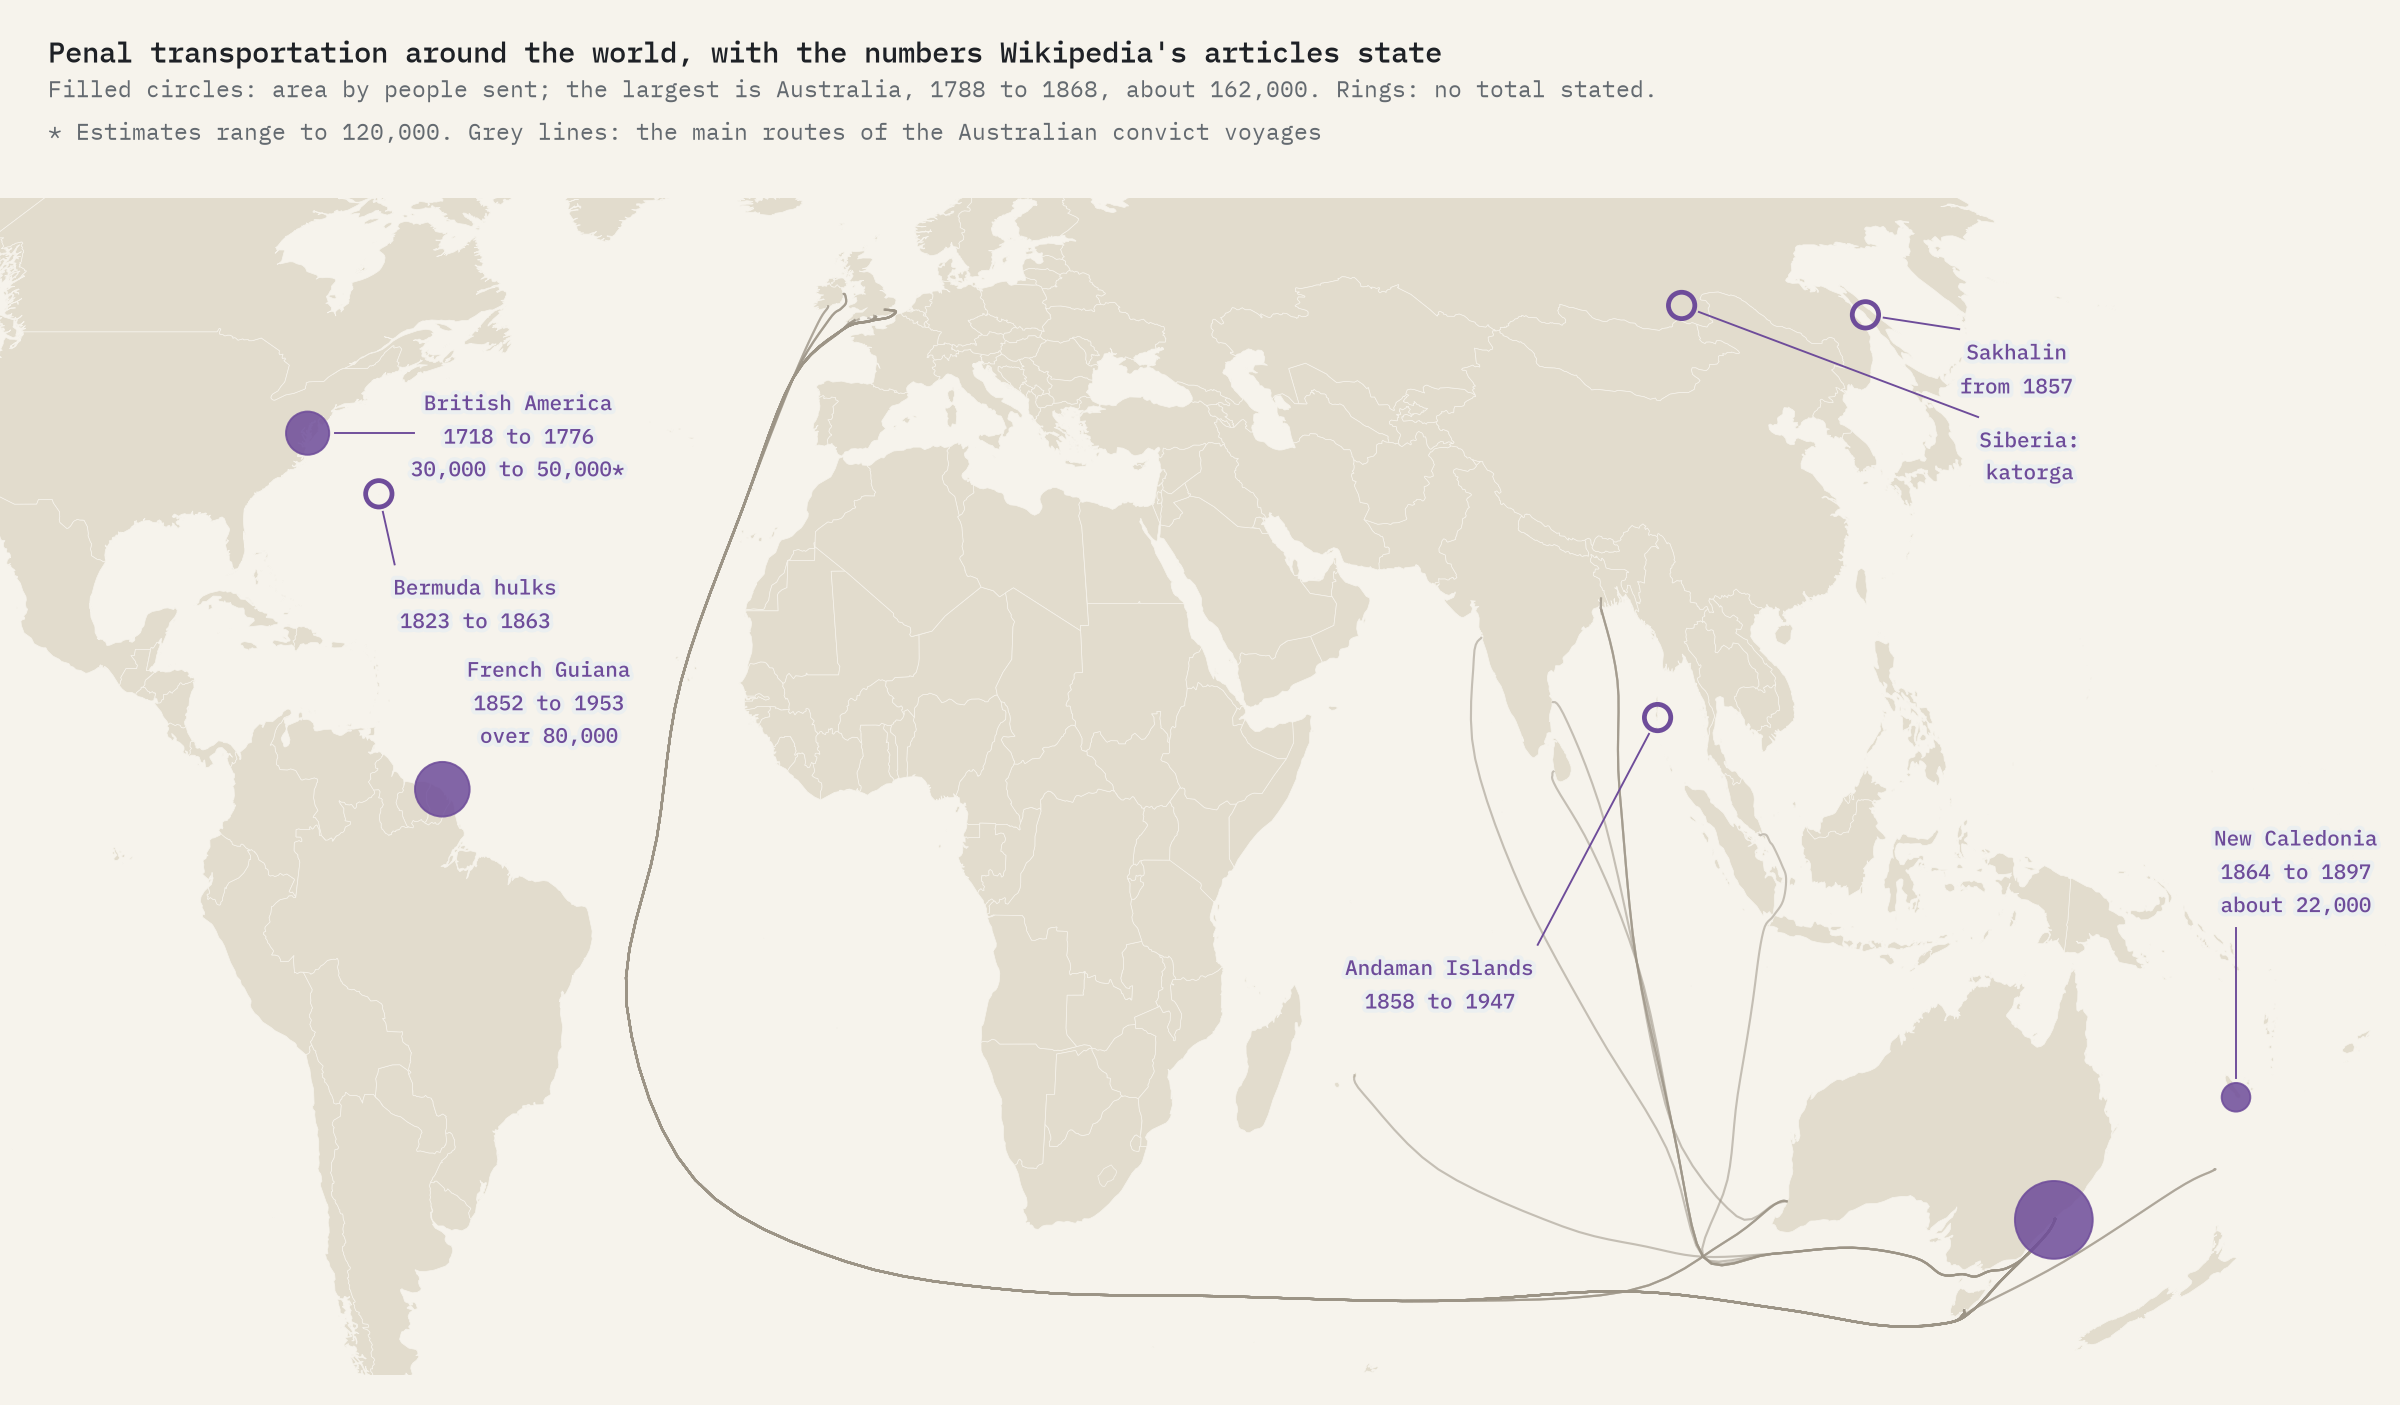
\includegraphics[width=\textwidth]{f_world.png}
\caption{Penal transportation around the world, with the numbers the articles state.}\label{fig:world}\end{figure}

\section{Limitations}
First, the lists are volunteer compilations, mostly from Bateson, and have not been checked here against primary records; the Tasmania list in particular is short for the traffic it describes and stops a year before the last voyage its introduction names. Second, they give convict numbers for under a sixth of the voyages, so the people transported cannot be counted from them. Third, the duration and death samples are small and drawn from the best documented ships. Fourth, duplicate detection across lists is a rule of thumb. Fifth, the routes are stylised. Sixth, the women's count is a floor. Finally, figures for other systems are what the articles state, and their sources vary.

\section{Conclusion}
Wikipedia's lists are a good guide to the convict shipping of the Australian colonies: when it came, where it sailed from and how its rhythm shifted from Sydney to Hobart, Norfolk Island and Fremantle. They are a poor guide to the people on board. The voyages they describe carried people far from home, onto land taken from Aboriginal nations, and they belong to a wider history of empires exiling their convicts, from the Chesapeake to Sakhalin.

\section*{Data and code availability}
The interactive map is at \url{https://maps.tristanhotham.com/transported-convicts/}. Data and code are at \url{https://github.com/Tristan-Hotham/transported-convicts} and archived with this paper at https://doi.org/10.5281/zenodo.23873537. Code is released under the MIT licence; text and figures under CC BY 4.0; the tables derived from Wikipedia under CC BY-SA 4.0.

\section*{AI statement}
I wrote the text, with drafting and editing assistance from Claude (Anthropic), which also helped prepare the analysis code. I reviewed and checked all text and results.

\begin{table}[tbp]\centering\small\caption{English Wikipedia articles used, with the revision read (CC BY-SA 4.0). Also used, from a search dump without revision ids: Convict ship, Devil's Island, Penal colony, Port Blair, Sakhalin, Gulag, Andaman Islands, Hulk (ship type), and the full text of the convict ship articles named in the data.}\label{tab:revs}\begin{tabular}{lr}\toprule Article & Revision\\\midrule
Australian Convict Sites & 1366152364\\
Bagne (penal establishment) & 1378312137\\
Cellular Jail & 1379660571\\
Convict era of Western Australia & 1376677837\\
Convict ships to New South Wales & 1329275779\\
Convict ships to Norfolk Island & 1383115444\\
Convict ships to Tasmania & 1153506110\\
Convict women in Australia & 1346295726\\
Convicts in Australia & 1373855829\\
First Fleet & 1381165491\\
Indentured servitude in British America & 1368066200\\
Katorga & 1371129600\\
List of British prison hulks & 1379028118\\
List of convict ship voyages to Western Australia & 1334470026\\
List of convicts transported to Australia & 1369575880\\
Macquarie Harbour Penal Station & 1368436442\\
Moreton Bay Penal Settlement & 1376283471\\
Norfolk Island & 1381712229\\
Penal transportation & 1381060835\\
Port Arthur, Tasmania & 1381786866\\
Royal Naval Dockyard, Bermuda & 1377314982\\
Second Fleet (Australia) & 1339109887\\
Third Fleet (Australia) & 1308790478\\
Transportation Act 1717 & 1381752810\\
\bottomrule\end{tabular}\end{table}

\begin{thebibliography}{9}
\bibitem[Natural Earth(2026)]{naturalearth} Natural Earth (2026) Land and admin 0 countries (1:50m). Public domain. \url{https://www.naturalearthdata.com/}
\bibitem[Wikipedia(2026)]{wiki} Wikipedia contributors (2026) English Wikipedia articles listed in Table~\ref{tab:revs}, at the revisions given. CC BY-SA 4.0. \url{https://en.wikipedia.org/}
\end{thebibliography}
\end{document}
